\section*{What has been done this week}
%\textit{\textbf{Hint:}Try to write this section so it can be used directly in your thesis. Also use drawings and figures.}


\section{Choosing the best metric}
In this section, the four metrics will be given different parameters to make them perform their best.\footnote{\textcolor{red}{rewrite}}

\subsection{Tweaking parameters}
Some of the chosen metrics have constants that can be adjusted to optimize the correctness of the output scores. This concerns the histogram frequency-based and the frequency domain metrics.

The best possible constants have been chosen experimentally, looking at the AUC value of the outputs when running the metric on the training data set. The constants will be chosen between those that provide the highest AUC values on the training data set both including and excluding the Gaussian blurred images.

\subsubsection{HF}
In the histogram frequency-based metric, the two thresholds, $minDCTValue$ and $maxHistValue$, can be adjusted for optimizing the output.

\begin{figure}[H]
    \centering
    \begin{subfigure}[t]{0.48\textwidth}
        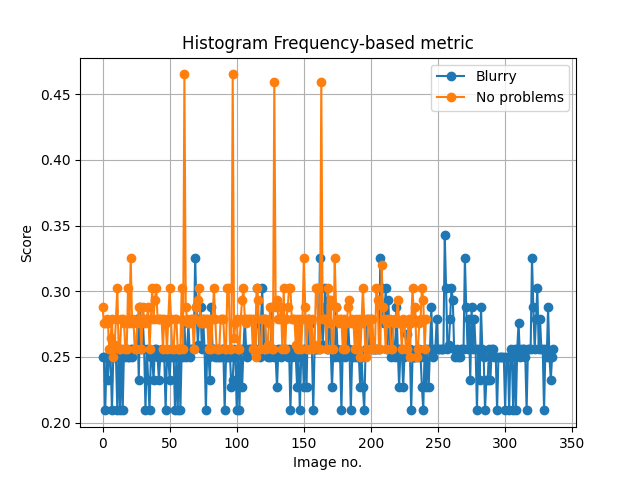
\includegraphics[width=\textwidth]{Figures/tweakHF/min1_max0.085_output_basic_no_gauss.png}
        \caption{}
        \label{fig:HF_basic_85}
    \end{subfigure}\hspace{1em}
    \begin{subfigure}[t]{0.48\textwidth}
        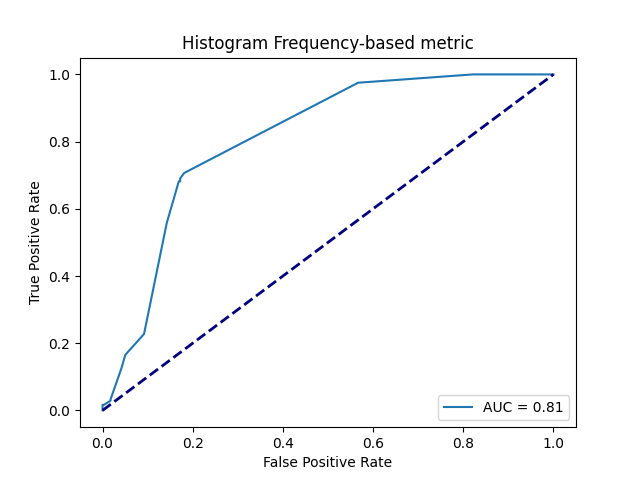
\includegraphics[width=\textwidth]{Figures/tweakHF/min1_max0.085_output_roc_no_gauss.png}
        \caption{One of the two best performances without Gauss have constants $minDCTValue=1$ and $maxHistValue=0.085$, having AUC$=0.81$.}
        \label{fig:HF_roc_85}
    \end{subfigure}\hspace{1em}
    \begin{subfigure}[t]{0.48\textwidth}
        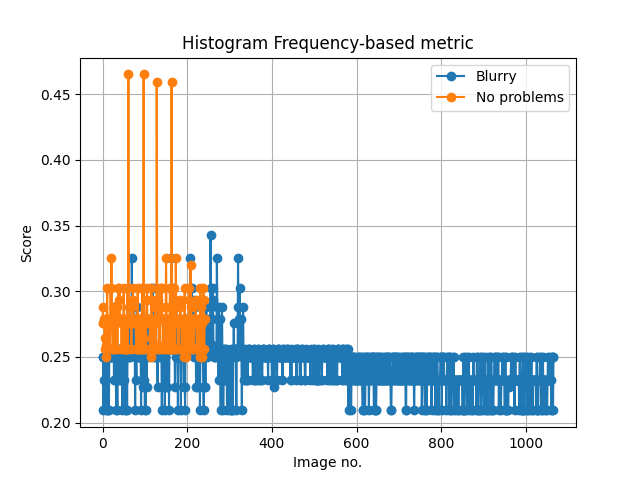
\includegraphics[width=\textwidth]{Figures/tweakHF/min1_max0.085_output_basic.png}
        \caption{}
        \label{fig:HF_basic_gauss_85}
    \end{subfigure}\hspace{1em}
    \begin{subfigure}[t]{0.48\textwidth}
        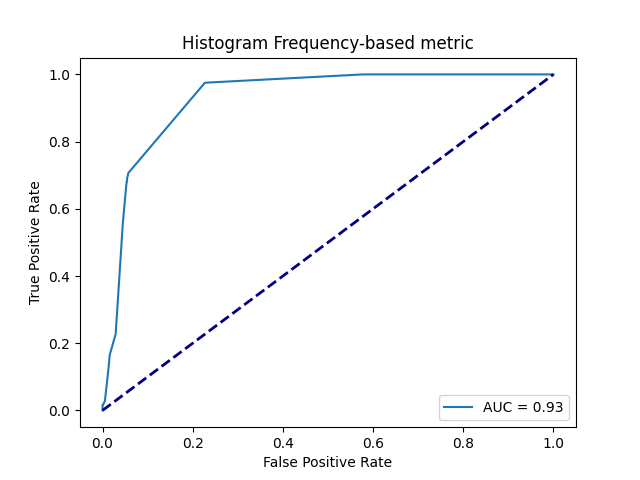
\includegraphics[width=\textwidth]{Figures/tweakHF/min1_max0.085_output_roc.png}
        \caption{The output on the training set including Gauss on constants $minDCTValue=1$ and $maxHistValue=0.085$, having AUC$=0.93$.}
        \label{fig:HF_roc_gauss_85}
    \end{subfigure}
    \caption{The output with $minDCTValue=1$ and $maxHistValue=0.085$.}
\end{figure}

\begin{figure}[H]
    \begin{subfigure}[t]{0.48\textwidth}
        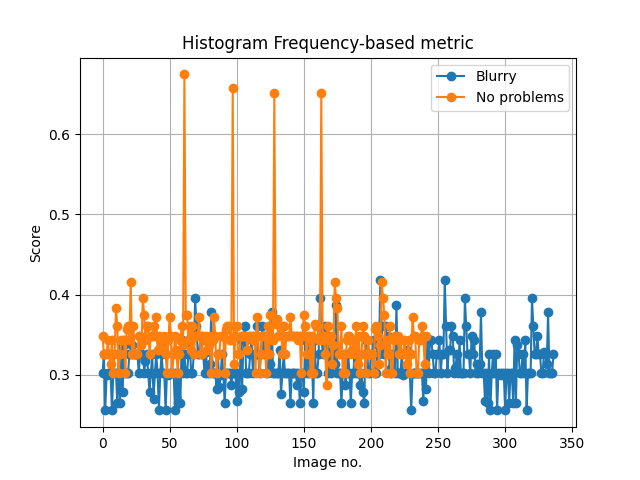
\includegraphics[width=\textwidth]{Figures/tweakHF/min0_max0.115_output_basic.png}
        \caption{}
        \label{fig:HF_basic_115}
    \end{subfigure}\hspace{1em}
    \begin{subfigure}[t]{0.48\textwidth}
        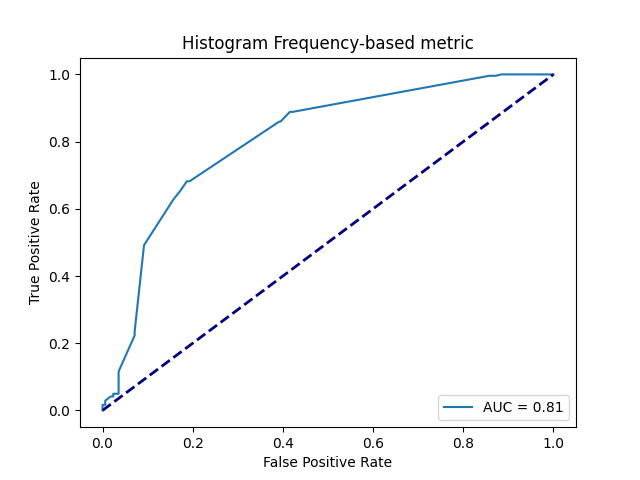
\includegraphics[width=\textwidth]{Figures/tweakHF/min0_max0.115_output_roc.png}
        \caption{One of the two best performances on the training set with $minDCTValue=0$, $maxHistValue=0.115$ and without Gauss, having AUC$=0.81$.}
        \label{fig:HF_roc_115}
    \end{subfigure}\hspace{1em}
    \begin{subfigure}[t]{0.48\textwidth}
        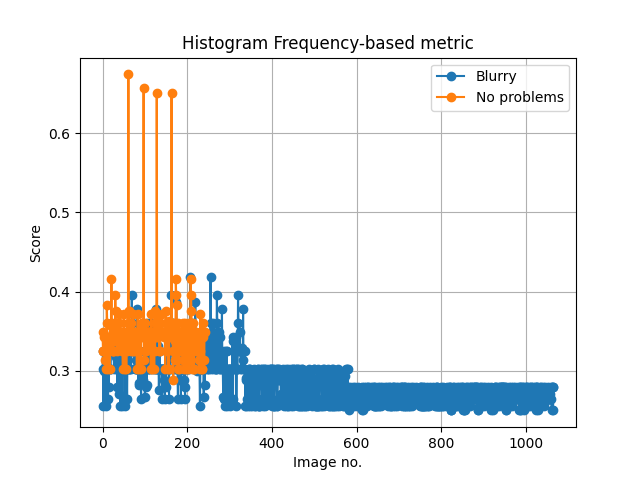
\includegraphics[width=\textwidth]{Figures/tweakHF/gauss_min0_max0.115_output_basic.png}
        \caption{}
        \label{fig:HF_basic_gauss_115}
    \end{subfigure}\hspace{1em}
    \begin{subfigure}[t]{0.48\textwidth}
        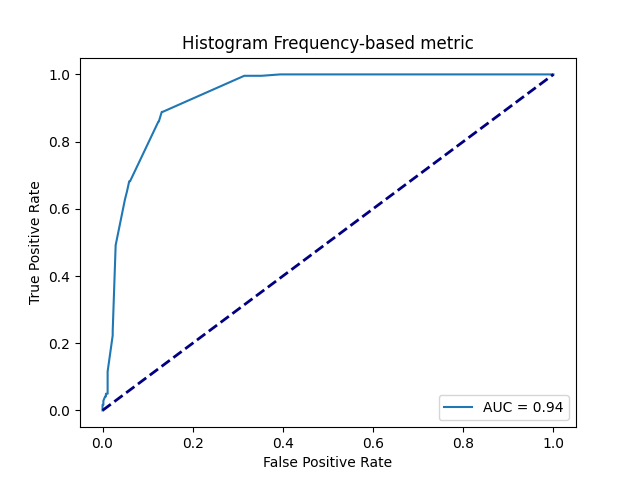
\includegraphics[width=\textwidth]{Figures/tweakHF/gauss_min0_max0.115_output_roc.png}
        \caption{The best performance with Gauss is with $minDCTValue=0$ and $maxHistValue=0.115$, having AUC$=0.94$.}
        \label{fig:HF_roc_gauss_115}
    \end{subfigure}
    \caption{The output with $minDCTValue=0$ and $maxHistValue=0.115$.}
    \label{fig:tweakHF}
\end{figure}
The correctness of the output of the algorithm doesn't seem to be distorted by the Gaussian blurred images. In figure \ref{fig:tweakHF} the ROC curves with highest scores are displayed. As can be seen, the output of running the algorithm on the training set without Gaussian blurred images performs very well in two different situations. The correctness is also very high and almost identical for the results including the Gaussian blurred images. However, it is a little better with the lower $minDCTValue=0$, whose purpose is filtering away noise. That is, when no noise is filtered away.

Knowing this, the $minDCTValue=1$ and $maxHistValue=0.085$ are chosen for the metric, as the purpose of the metric is not detecting Gaussian blur, but blur in non-manipulated images, where noise could occur, and as the worsening of the results on the Gaussian blurred images is insignificant.

%The Gaussian blurred images will not be used for training the metrics, as they distort the results. This can be seen in the above images, where the metric tend to perform excellent on the the training set including the Gaussian images, but not very well on the training set without. On the other hand, the metric performs well when given other parameters and the training set without Gauss.

\subsubsection{FM}
In the frequency domain image blur measure, the threshold $t=\dfrac{M}{1000}$ is experimentally estimated \footnote{\textit{Experimentally it is observed that this particular threshold value gives a fairly accurate sense of image quality}\cite{FM}}. This will also be done in the following, where the constant for division ($1000$) is varied.

\begin{figure}[H]
    \centering
    \begin{subfigure}[t]{0.48\textwidth}
        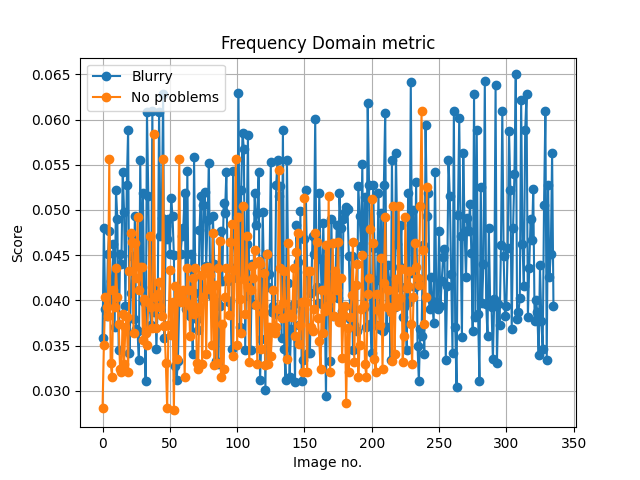
\includegraphics[width=\textwidth]{Figures/tweakFM/102_output_basic_no_gauss.png}
        \caption{}
        \label{fig:FM_basic_102}
    \end{subfigure}\hspace{1em}
    \begin{subfigure}[t]{0.48\textwidth}
        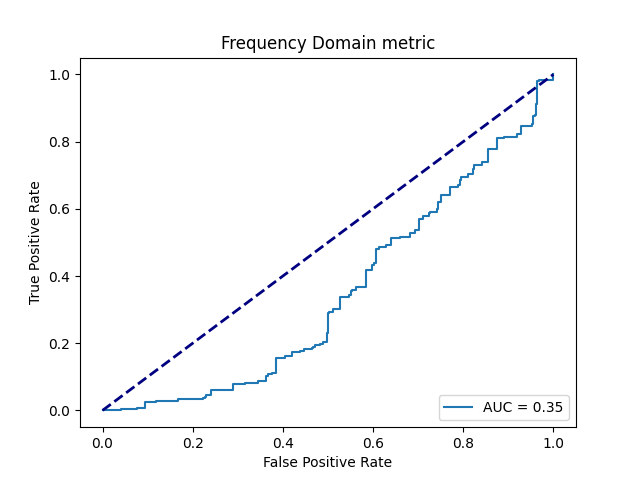
\includegraphics[width=\textwidth]{Figures/tweakFM/102_output_roc_no_gauss.png}
        \caption{The worst performance with constant $102$ and no Gauss, having AUC$=0.35$.}
        \label{fig:FM_roc_102}
    \end{subfigure}\hspace{1em}
    \begin{subfigure}[t]{0.48\textwidth}
        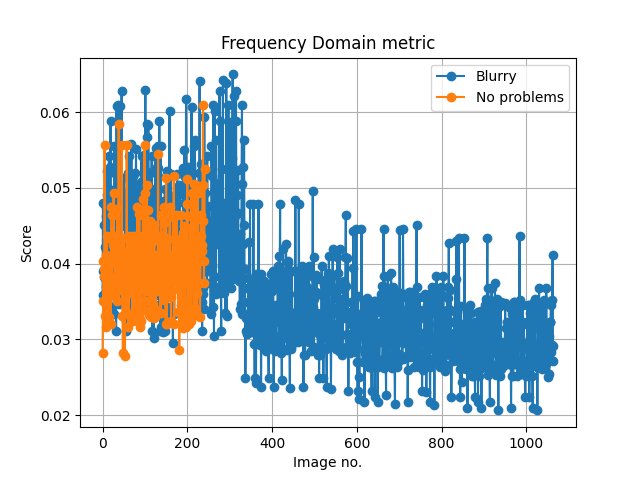
\includegraphics[width=\textwidth]{Figures/tweakFM/102_output_basic.png}
        \caption{}
        \label{fig:FM_basic_gauss_102}
    \end{subfigure}\hspace{1em}
    \begin{subfigure}[t]{0.48\textwidth}
        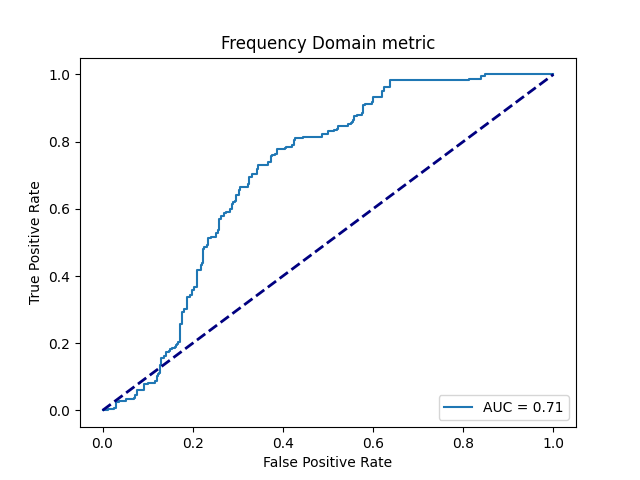
\includegraphics[width=\textwidth]{Figures/tweakFM/102_output_roc.png}
        \caption{The performance with constant $102$ on the training set including Gauss, having AUC$=0.71$.}
        \label{fig:FM_roc_gauss_102}
    \end{subfigure}
    \caption{The output with a constant of value $102$}
\end{figure}

\begin{figure}[H]
    \begin{subfigure}[t]{0.48\textwidth}
        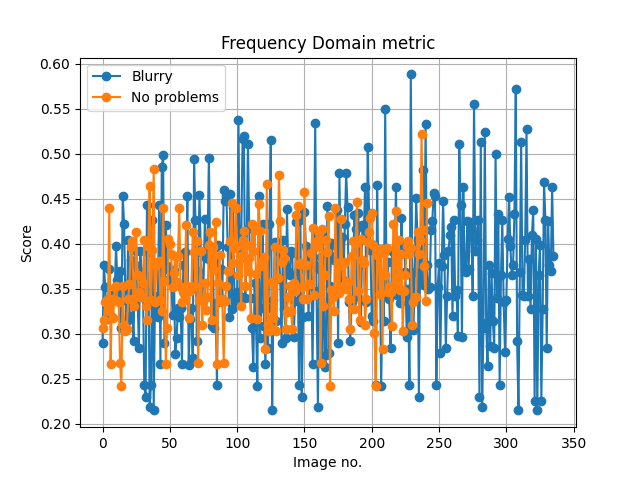
\includegraphics[width=\textwidth]{Figures/tweakFM/2202_output_basic.png}
        \caption{}
        \label{fig:FM_basic_2202}
    \end{subfigure}\hspace{1em}
    \begin{subfigure}[t]{0.48\textwidth}
        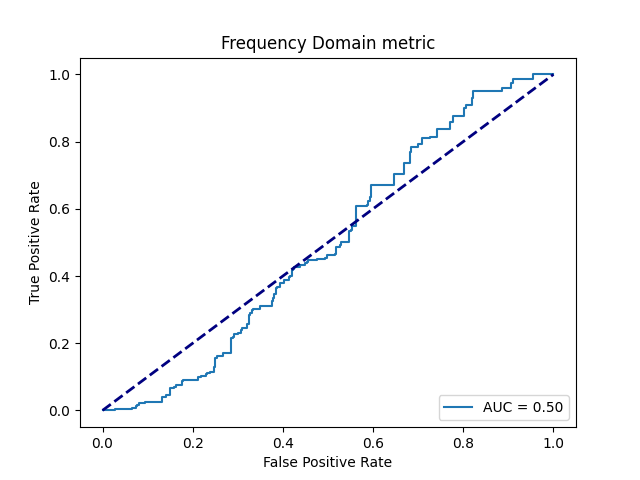
\includegraphics[width=\textwidth]{Figures/tweakFM/2202_output_roc.png}
        \caption{The AUC$=0.5$ on the training set without Gauss with the constant $2202$.}
        \label{fig:FM_roc_2202}
    \end{subfigure}\hspace{1em}
    \begin{subfigure}[t]{0.48\textwidth}
        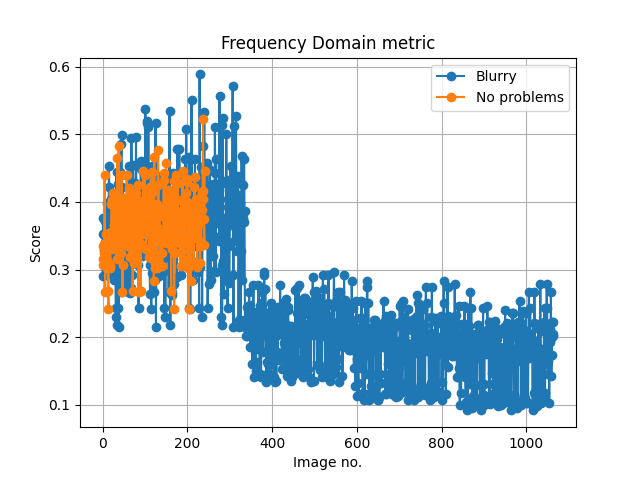
\includegraphics[width=\textwidth]{Figures/tweakFM/2202_output_basic_gauss.png}
        \caption{}
        \label{fig:FM_basic_gauss_2202}
    \end{subfigure}\hspace{1em}
    \begin{subfigure}[t]{0.48\textwidth}
        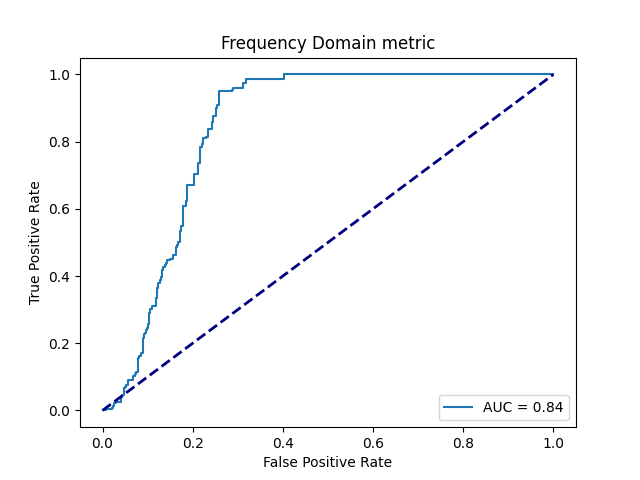
\includegraphics[width=\textwidth]{Figures/tweakFM/2202_output_roc_gauss.png}
        \caption{One of the best performances with Gauss is with the constant $2202$, having AUC$=0.84$.}
        \label{fig:FM_roc_gauss_2202}
    \end{subfigure}
    \caption{The output with a constant of value $2202$}
\end{figure}
The Gaussian blurred images will not be taking into account when choosing the constant for the metric, as they distort the result. This can be seen in the above images, where the metric performs excellent on the training set including the Gaussian images, while at the same time it performs quite badly on the training set without. The AUC in the tests on the training set without Gauss did not manage to exceed $53\%$, however, the lowest value was $35\%$, which gives an AUC of $100\%-35\%=65\%$. However, doing this, the metric would classify the Gaussian blurred images as sharper when applying more blur.

As this metric performs worst of all 4, it will not be taken into account in the following sections.

% \subsubsection{CPBD}
% The cumulative probability of blur detection metric has a threshold that classifies a block as smooth if the number of edge pixels in the block is below $0.2\%$ of the pixels in the whole block.
% theta can't be estimated, as we do not have the data for it...
% \textit{In (1), the values of and are chosen, by means of a least-square fitting, to increase the correspondence of (1) with the experimentally determined psychometric function (given by the normalized histogram of the subjects’ responses).\cite{JNB}}


\subsection{"Training" the metrics}
The goal is to avoid false positives (\textbf{FP}: classified as sharp when blurry), as these can distort the results from the data later on, while still achieving some positive outputs.

\textbf{Choosing the threshold:}\\
Let the user choose an acceptable TNR (specificity), e.g. 98\%.\\
After this, find the corresponding threshold and choose the metric with the highest accuracy, as it will provide a possibility that some images will be "accepted", that is, classified as sharp. 

We could also calculate summed distance, d, of some rates... TPR (sensitivity), F1-score, precision...  to the top and bottom border (1 and 0) according to which border is desired for that particular rate. Then choose the metric with smallest d.


\begin{itemize}
    % \item minimize FPR (sharp when not) ($1-TNR$)
    \item maximize TNR (how many are blurry when blurry)
    \item maximize TPR (we would still like some possibility that images are classified "sharp")
    \item maximize PPV (part declared sharp when sharp)
    \item high f1-score for general score + do not produce FP (to not filter away too many negatives)
\end{itemize}


The following graphs displays output on the training data set excluding the Gaussian blurred images.



\subsection{CPBD}
\begin{figure}[H]
    \centering
    \begin{subfigure}[t]{0.48\textwidth}
        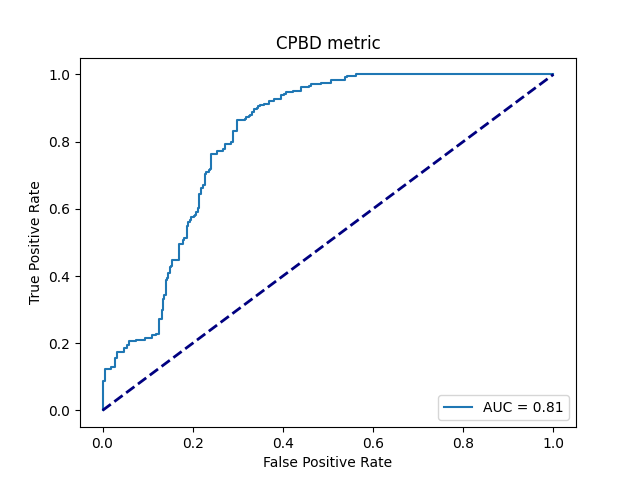
\includegraphics[width=\textwidth]{Figures/results_on_thresholds/output_roc_cpbd.png}
        \caption{}
        \label{fig:CPBD_roc}
    \end{subfigure}\hspace{1em}
    \begin{subfigure}[t]{0.48\textwidth}
        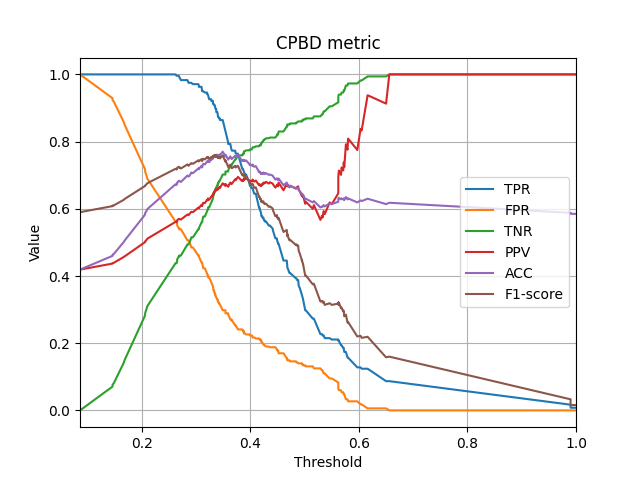
\includegraphics[width=\textwidth]{Figures/results_on_thresholds/threshold_test_scores_cpbd.png}
        \caption{}
        \label{fig:CPBD_thresh}
    \end{subfigure}\hspace{1em}
    \begin{subfigure}[t]{0.48\textwidth}
        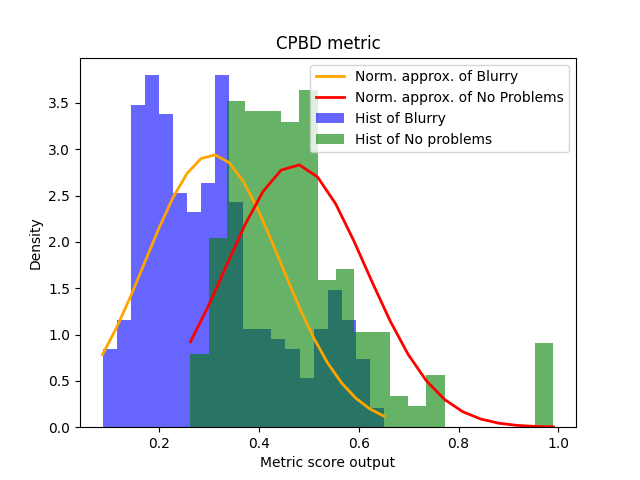
\includegraphics[width=\textwidth]{Figures/results_on_thresholds/output_dens_cpbd.png}
        \caption{}
        \label{fig:CPBD_dens}
    \end{subfigure}\hspace{1em}
    \caption{}
    \label{fig:CPBD_final}
\end{figure}

\subsection{Variance of Laplacian}
\begin{figure}[H]
    \centering
    \begin{subfigure}[t]{0.48\textwidth}
        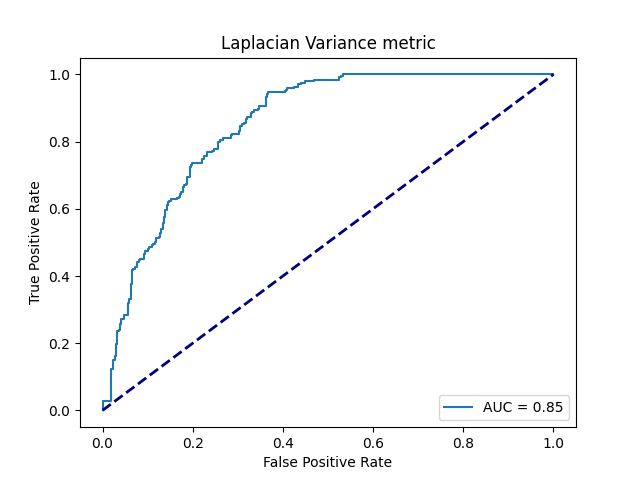
\includegraphics[width=\textwidth]{Figures/results_on_thresholds/output_roc_lv.png}
        \caption{}
        \label{fig:LV_roc}
    \end{subfigure}\hspace{1em}
    \begin{subfigure}[t]{0.48\textwidth}
        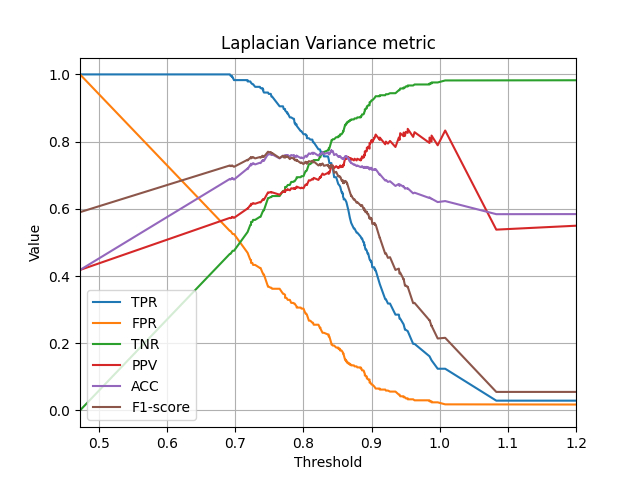
\includegraphics[width=\textwidth]{Figures/results_on_thresholds/threshold_test_scores_lv.png}
        \caption{}
        \label{fig:LV_thresh}
    \end{subfigure}\hspace{1em}
    \begin{subfigure}[t]{0.48\textwidth}
        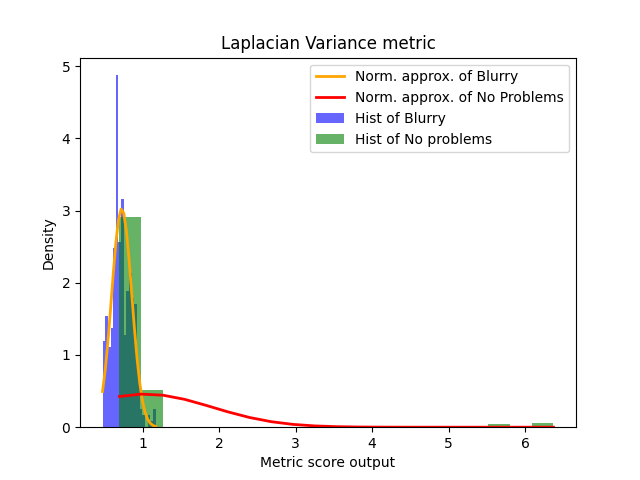
\includegraphics[width=\textwidth]{Figures/results_on_thresholds/output_dens_lv.png}
        \caption{}
        \label{fig:LV_dens}
    \end{subfigure}\hspace{1em}
    \caption{}
    \label{fig:LV_final}
\end{figure}

\subsection{Histogram frequency-based metric}
\begin{figure}[H]
    \centering
    \begin{subfigure}[t]{0.48\textwidth}
        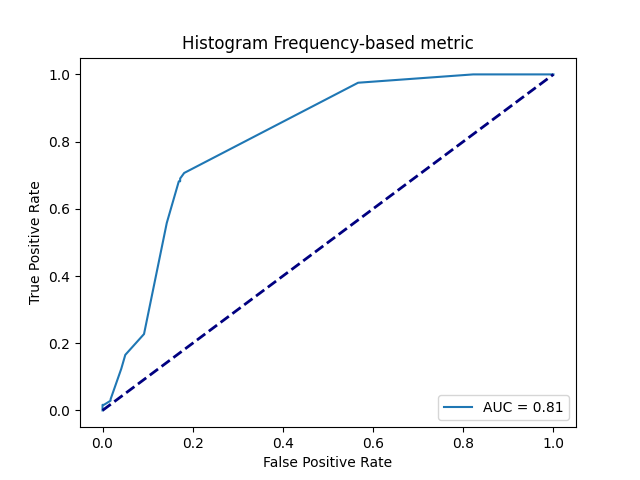
\includegraphics[width=\textwidth]{Figures/results_on_thresholds/output_roc_hf.png}
        \caption{}
        \label{fig:HF_roc}
    \end{subfigure}\hspace{1em}
    \begin{subfigure}[t]{0.48\textwidth}
        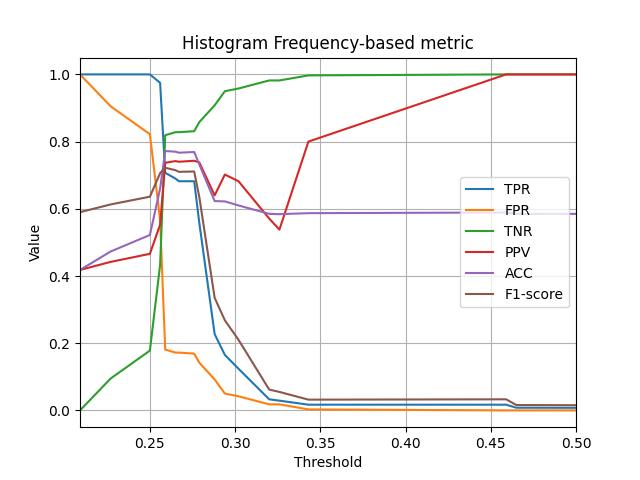
\includegraphics[width=\textwidth]{Figures/results_on_thresholds/threshold_test_scores_hf.png}
        \caption{}
        \label{fig:HF_thresh}
    \end{subfigure}\hspace{1em}
    \begin{subfigure}[t]{0.48\textwidth}
        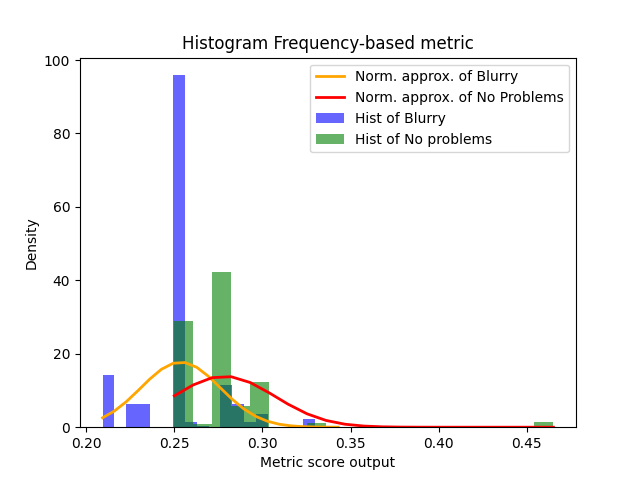
\includegraphics[width=\textwidth]{Figures/results_on_thresholds/output_dens_hf.png}
        \caption{}
        \label{fig:HF_dens}
    \end{subfigure}\hspace{1em}
    \caption{}
    \label{fig:HF_final}
\end{figure}

\subsection{Merge of CPBD and Variance of Laplacian}
\textbf{Highest AUC = 90\%}
\begin{figure}[H]
    \centering
    \begin{subfigure}[t]{0.48\textwidth}
        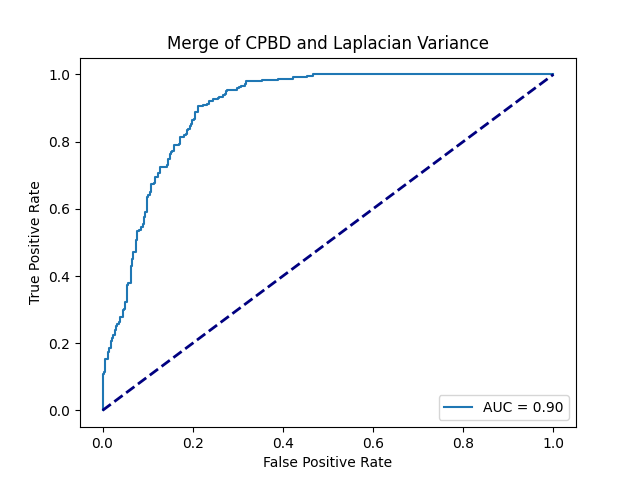
\includegraphics[width=\textwidth]{Figures/results_on_thresholds/output_roc_cpbd_lv.png}
        \caption{}
        \label{fig:CPBD_LV_roc}
    \end{subfigure}\hspace{1em}
    \begin{subfigure}[t]{0.48\textwidth}
        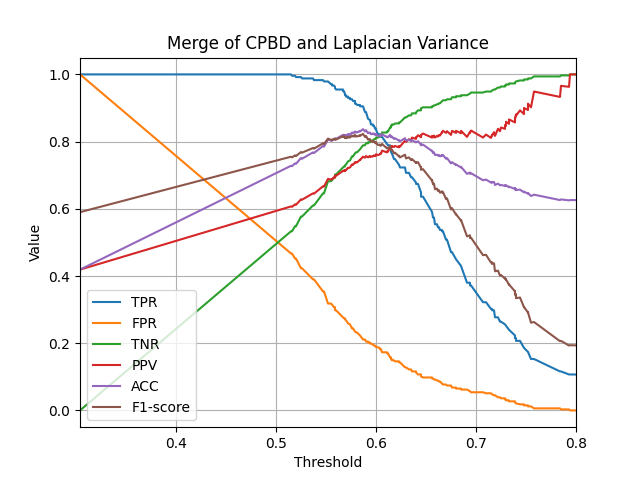
\includegraphics[width=\textwidth]{Figures/results_on_thresholds/threshold_test_scores_cpbd_lv.png}
        \caption{}
        \label{fig:CPBD_LV_thresh}
    \end{subfigure}\hspace{1em}
    \begin{subfigure}[t]{0.48\textwidth}
        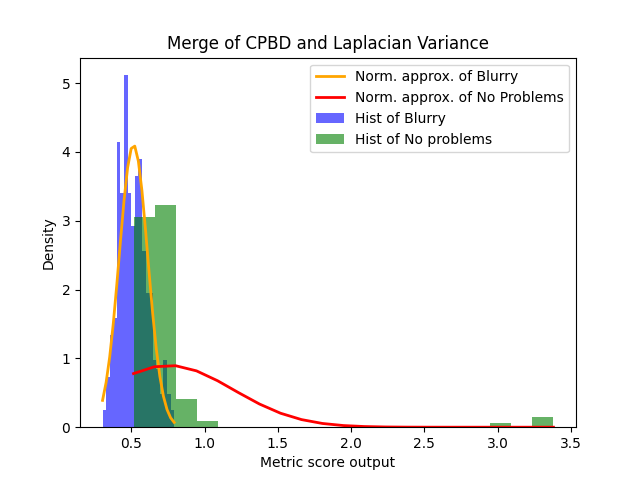
\includegraphics[width=\textwidth]{Figures/results_on_thresholds/output_dens_cpbd_lv.png}
        \caption{}
        \label{fig:CPBD_LV_dens}
    \end{subfigure}\hspace{1em}
    \caption{}
    \label{fig:CPBD_LV_final}
\end{figure}

\subsection{Merge of CPBD and Histogram frequency-based metric}
\begin{figure}[H]
    \centering
    \begin{subfigure}[t]{0.48\textwidth}
        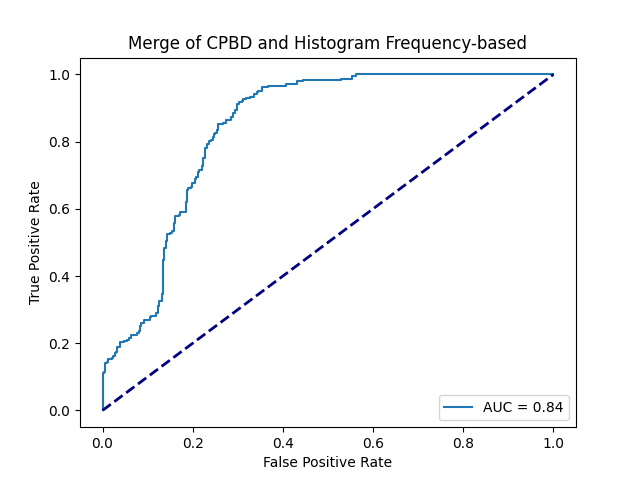
\includegraphics[width=\textwidth]{Figures/results_on_thresholds/output_roc_cpbd_hf.png}
        \caption{}
        \label{fig:CPBD_HF_roc}
    \end{subfigure}\hspace{1em}
    \begin{subfigure}[t]{0.48\textwidth}
        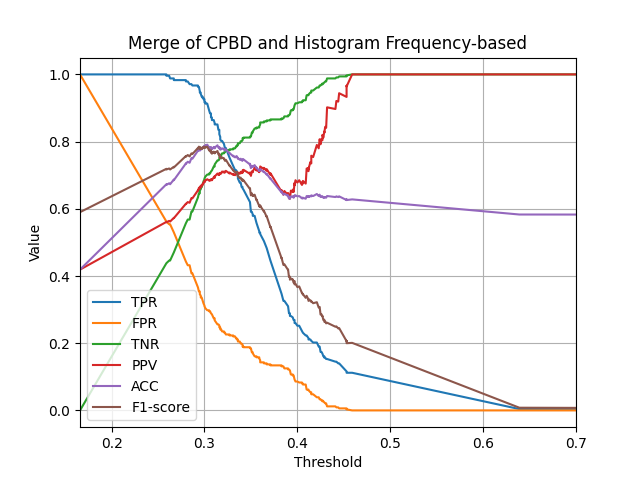
\includegraphics[width=\textwidth]{Figures/results_on_thresholds/threshold_test_scores_cpbd_hf.png}
        \caption{}
        \label{fig:CPBD_HF_thresh}
    \end{subfigure}\hspace{1em}
    \begin{subfigure}[t]{0.48\textwidth}
        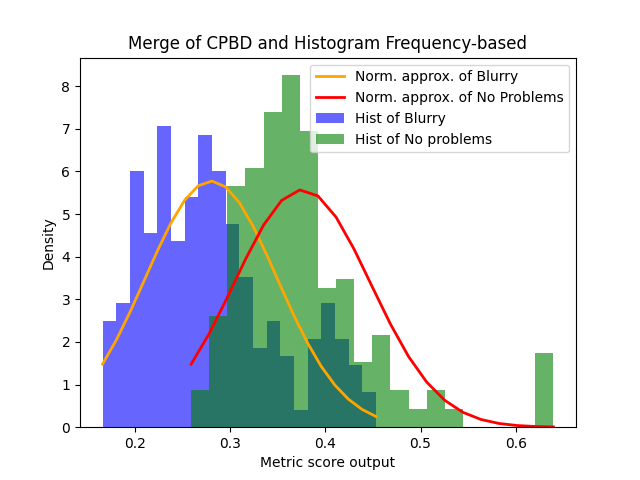
\includegraphics[width=\textwidth]{Figures/results_on_thresholds/output_dens_cpbd_hf.png}
        \caption{}
        \label{fig:CPBD_HF_dens}
    \end{subfigure}\hspace{1em}
    \caption{}
    \label{fig:CPBD_HF_final}
\end{figure}

\subsection{Merge of Histogram frequency-based metric and Variance of Laplacian}
\begin{figure}[H]
    \centering
    \begin{subfigure}[t]{0.48\textwidth}
        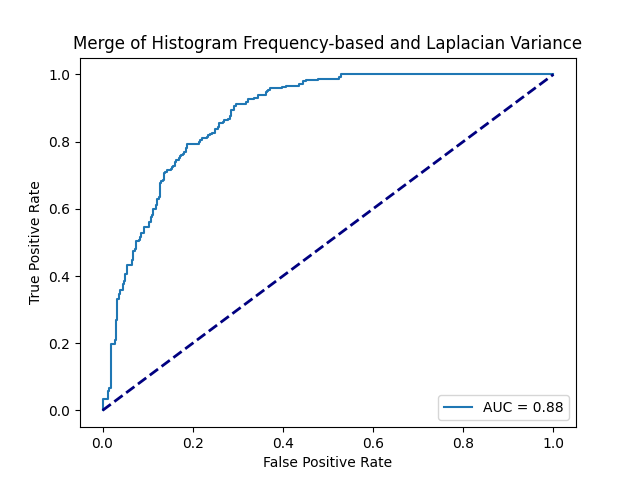
\includegraphics[width=\textwidth]{Figures/results_on_thresholds/output_roc_hf_lv.png}
        \caption{}
        \label{fig:HF_LV_roc}
    \end{subfigure}\hspace{1em}
    \begin{subfigure}[t]{0.48\textwidth}
        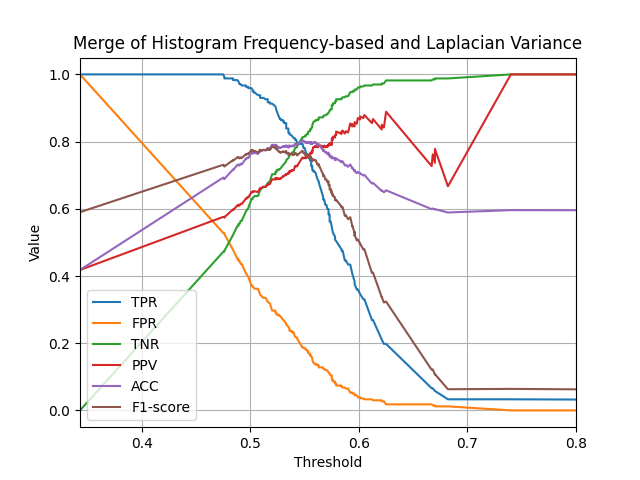
\includegraphics[width=\textwidth]{Figures/results_on_thresholds/threshold_test_scores_hf_lv.png}
        \caption{}
        \label{fig:HF_LV_thresh}
    \end{subfigure}\hspace{1em}
    \begin{subfigure}[t]{0.48\textwidth}
        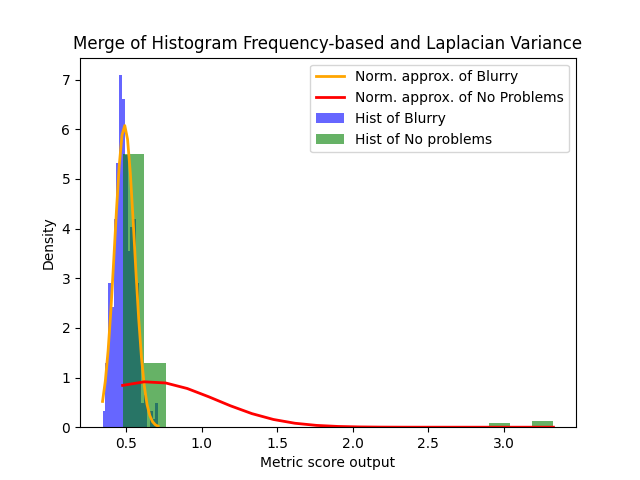
\includegraphics[width=\textwidth]{Figures/results_on_thresholds/output_dens_hf_lv.png}
        \caption{}
        \label{fig:HF_LV_dens}
    \end{subfigure}\hspace{1em}
    \caption{}
    \label{fig:HF_LV_final}
\end{figure}

\subsection{Merge of CPBD, Histogram frequency-based metric and Variance of Laplacian}
\begin{figure}[H]
    \centering
    \begin{subfigure}[t]{0.48\textwidth}
        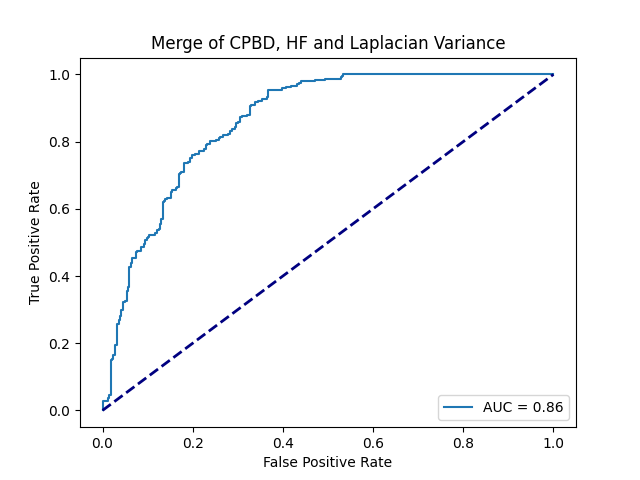
\includegraphics[width=\textwidth]{Figures/results_on_thresholds/output_roc_cpbd_hf_lv.png}
        \caption{}
        \label{fig:CPBD_HF_LV_roc}
    \end{subfigure}\hspace{1em}
    \begin{subfigure}[t]{0.48\textwidth}
        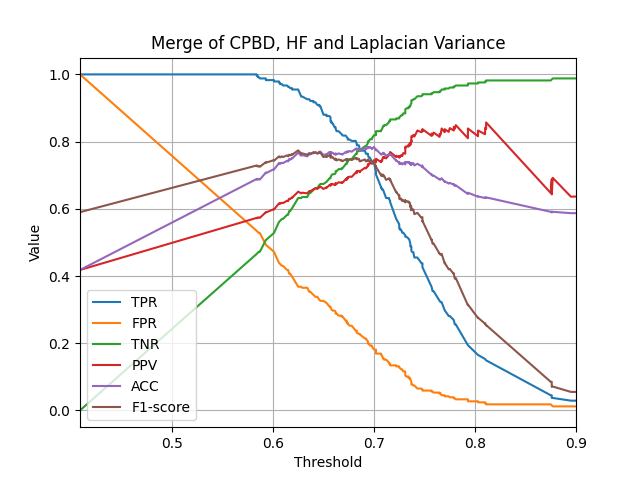
\includegraphics[width=\textwidth]{Figures/results_on_thresholds/threshold_test_scores_cpbd_hf_lv.png}
        \caption{}
        \label{fig:CPBD_HF_LV_thresh}
    \end{subfigure}\hspace{1em}
    \begin{subfigure}[t]{0.48\textwidth}
        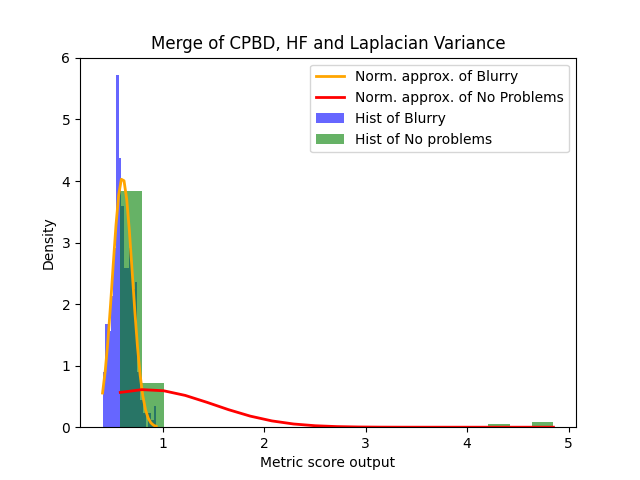
\includegraphics[width=\textwidth]{Figures/results_on_thresholds/output_dens_cpbd_hf_lv.png}
        \caption{}
        \label{fig:CPBD_HF_LV_dens}
    \end{subfigure}\hspace{1em}
    \caption{}
    \label{fig:CPBD_HF_LV_final}
\end{figure}


